\section{Аутентификация} \label{sec:authorization}
	Для аутентификации необходимо нажать на значок \vcenteredinclude[height=25px]{images/authorization/log_in_button} в верхнем правом углу страницы, после чего произойдёт перенаправление на страницу аутентификации (рис.~\ref{img:authorization:authorization_page}), где необходимо ввести свой логин (или адрес электронной почты) и пароль от учётной записи, после чего нажать на кнопку \vcenteredinclude[height=25px]{images/authorization/login_btn}.
	\begin{figure}[H]
		\center{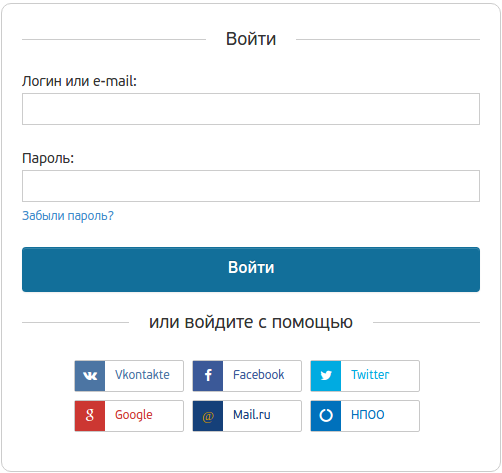
\includegraphics[height=9cm]{images/authorization/authorization_page}}
		\caption{Окно аутентификации}
		\label{img:authorization:authorization_page}
	\end{figure}
	
	В случае успеха пользователь будет перенаправлен на главную страницу Платформы, в противном случае (например, если пользователь ввёл неправильный пароль), пользователь увидит сообщение об ошибке.